% In dit onderdeel bespreek je een doordachte selectie van uitgevoerde activiteiten. Maak hierbij gebruik van de STARRT-methode.

% \begin{outline}
%   \1 Omschrijving
%     \2 Doelstelling(en) van de activiteit
%     \2 Eigen doelstelling(en)
%     \2 Optioneel teamsamenstelling (taakverdeling)
%   \1 Kern (showcase): min 500 woorden
%     \2 Verslag van de activiteit
%     \2 + screenshots, foto's, beeldmateriaal, \dots
%   \1 Reflectie opdracht: min 250 woorden
%     \2 Wat heb je gedaan?
%     \2 Heb je problemen ondervonden? Hoe heb je die aangemakt?
%     \2 Wat vond je ervan, hoe heb je het ervaren?
%     \2 Wat heb je geleerd?
%     \2 Wat waren jouw sterkte/zwakke punten?
%     \2 Wat zijn mogelijke linken met de opleiding?
%     \2 Waarom heb je deze opdracht geselecteerd voor de bespreking in jouw portfolio
% \end{outline}

% http://www.profi-leren.nl/files/oa_dc51.pdf

\subsection{Care\hyp{}athon - Ambulance Wens}
% https://pxl-digital.pxl.be/page/care-athon-2020#

De tweedaagse hackathon werd georganiseerd op de Corda Campus in gebouw 3 bij Cegeka. We werden hier ontvangen door Tristan Fransen en Francis Vos, die ons een korte introductie gaf over het onderwerp. Vervolgens maakten we kennis met de twee vertegenwoordigers van Ambulance Wens en Arno Barzan, de PXL\hyp{}begeleider van dit project. Arno Barzan gaf ons meer specifieke uitleg over wat er precies gerealiseerd moest worden en op welke manier. Mijn willekeurig ingedeelde team bestond uit vier studenten van applicatieontwikkeling en één systeem\hyp{} en netwerkbeheerder.

Ik heb gekozen voor de uitdaging van Ambulance Wens. Dit is een vzw die zich inzet voor mensen met een ongeneeslijke ziekte, die niet mobiel zijn en voelen dat hun heengaan nabij komt. Ze zorgen dat deze mensen hun laatste wens nog in vervulling kunnen brengen met de nodige medische ondersteuning. Zo kunnen ze een laatste keer met volle teugen genieten van het leven.

Omdat de interne organisatie en het tentoonstellen van wensen wat ouderwets was en stroef verliep, kregen wij de opdracht om een mobiele applicatie te ontwerpen voor de vzw. Aan de hand van deze app konden de pati"enten een wens kiezen en werd al het benodigd materiaal en personeel verzameld om te laten deelnemen aan deze wens. De nadruk lag dus vooral op de gebruiksvriendelijkheid en de consistentie van de applicatie.

Toen de hackathon daadwerkelijk van start ging, zijn we begonnen een taakverdeling in ons team, om de effici"entie van ons werk te vergroten. Zo focuste één student zich vooral op het maken van de mock\hyp{}ups, twee studenten op het onderzoek naar realiseerbaarheid en restricties van buitenaf en de overige twee studenten begonnen reeds met het ontwikkelen van de applicatie. Ik was één van die laatste twee, maar daarnaast hielp ik ook met het nemen van beslissingen in verband met de mock\hyp{}ups. De applicatie werd geschreven voor Android in Android Studio met Java als programmeertaal. De mock\hyp{}ups werden uitgewerkt in de webapplicatie van Marvel.

Rond het einde van de eerste dag zijn we als team tot het besluit gekomen dat we geen volledig uitgewerkte applicatie konden aanmaken in de voorziene tijd. Daarom zijn we gedurende de tweede dag ons meer gaan focussen op het afwerken en verfijnen van de mock\hyp{}ups, omdat we het idee naar voren brengen belangrijker vonden dan het afleveren van een half afgewerkt product. Op dat moment hebben we de taakverdeling opnieuw herschikt en zijn we dus met drie studenten aan de slag gegaan met de mock\hyp{}ups, terwijl de andere twee studenten verder onderzoek uitvoerden naar elementen als server hosting en GDPR\hyp{}wetgeving.

\begin{figure}[!h]
  \centering
  \begin{subfigure}[h]{0.3\textwidth}
    \centering
    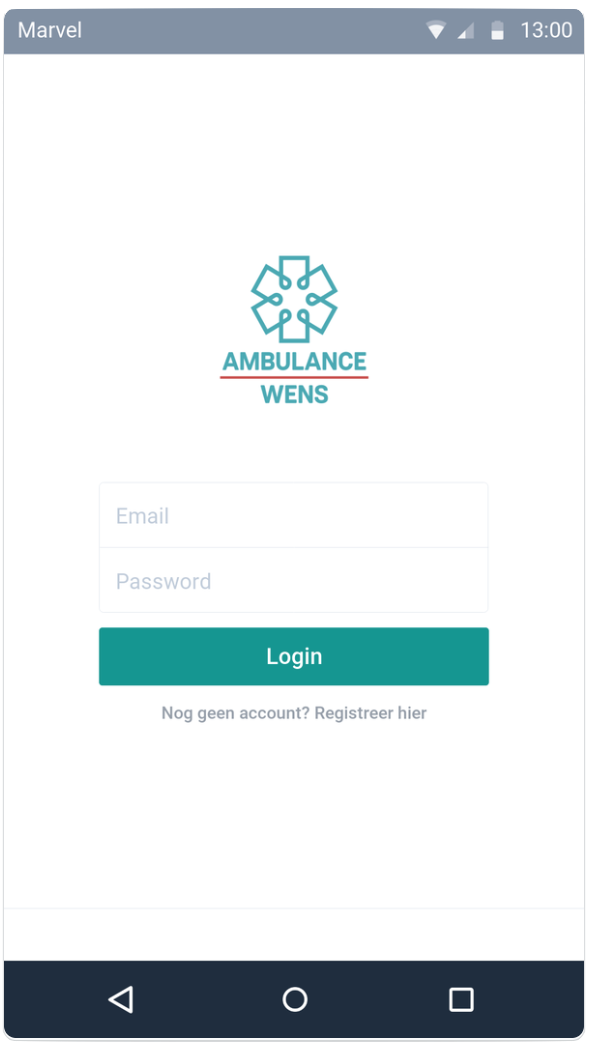
\includegraphics[width=0.76\textwidth]{images/care-athon/login.png}
  \end{subfigure}
  \begin{subfigure}[h]{0.3\textwidth}
    \centering
    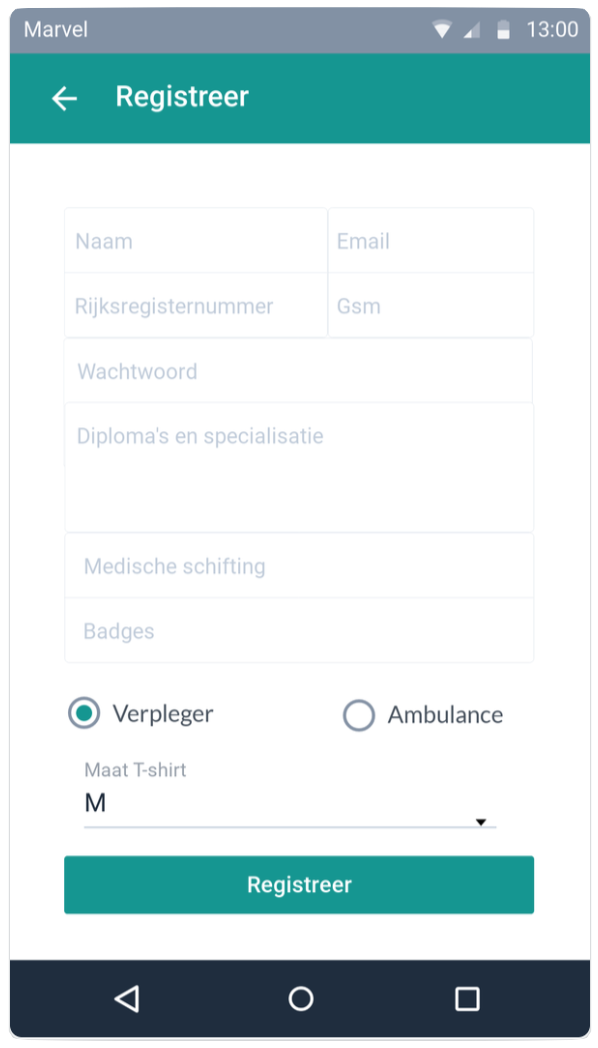
\includegraphics[width=0.76\textwidth]{images/care-athon/registreer.png}
  \end{subfigure}
  \begin{subfigure}[h]{0.3\textwidth}
    \centering
    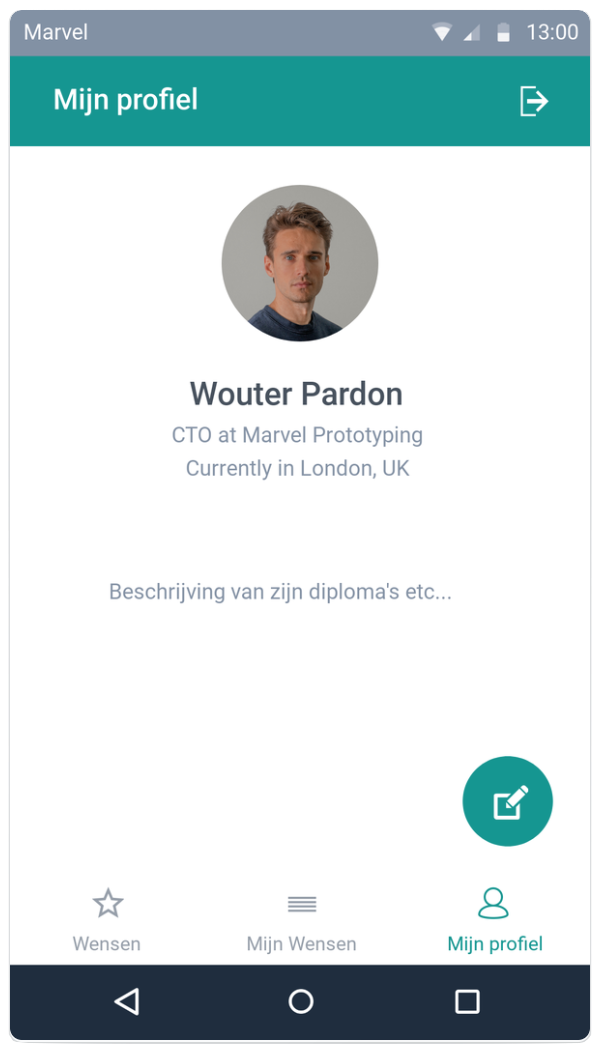
\includegraphics[width=0.76\textwidth]{images/care-athon/profiel.png}
  \end{subfigure}
\end{figure}

We konden op regelmatige basis feedback gaan vragen aan Arno Barzan en de twee vertegenwoordigers van Ambulance Wens, hetgeen ons meer inspiratie en duidelijkheid gaf over de opdracht, met een positief gevolg op onze applicatie. Zo wisten we welke informatie van de pati"enten, vrijwilligers en verplegers nodig was om de wens uit te kunnen voeren, en konden we het opvragen van deze info ook in onze applicatie verwerken. Anderzijds kregen we op die manier ook een beter idee over stijl waarin zij het liefst hun applicatie gezien hadden.

Op het einde van de hackaton presenteerde elke groep zijn applicatie voor de medestudenten, ook die van de andere uitdagingen. Onze presentatie was een demo van de applicatie aan de hand van de mock\hyp{}ups. Aangezien we ons onderzoek ook aan Ambulance Wens wilden overhandigen, hadden we een document gemaakt met alle gevonden informatie alsook onze mening over bepaalde beslissingen die gemaakt moesten worden.

Aan het einde van de hackathon kwam iedereen die hieraan deelnam samen in een aula om te luisteren naar verschillende sprekers. Daarop volgend waren de presentaties van alle teams. Na deze presentaties volgde de nominatie van de winnaars van elke uitdaging. Zij ontvingen een prijs afhankelijk van hun gekozen uitdaging.

Ik heb veel praktische zaken bijgeleerd van deze hackathon, zoals het maken van mock\hyp{}ups en het ontwikkelen van een applicatie met zeer specifieke restricties. Nooit voordien had ik zo een sterke nadruk gelegd op het maken van mock\hyp{}ups. Dit leerde ik van de student applicatieontwikkeling met full\hyp{}stack development als keuzetraject. Maar ook het feit dat we dermate moesten nadenken over het uitzicht van de applicatie in combinatie met de grote hoeveelheid eisen en restricties, heeft mijn visie over bepaalde aspecten van het ontwerp en de ontwikkeling zelf van projecten sterk be"invloed.

Daarnaast was de deelname aan een hackathon op zich ook nieuw voor mij. Het was een zeer verruimende ervaring, die mij op een zeer korte tijd in team veel nieuwe dingen over het uitwerken van een applicatie heeft bijgeleerd. Ik vind dat deze opdracht zeker een bijdrage heeft geleverd aan mijn opleiding en ik ben dus ook van mening dat dit in de opleiding vervat zou moeten blijven. Daarnaast heeft het mij ook doen inzien wat een software\hyp{}manager kan betekenen voor een team, omdat deze functie in ons team ontbrak en ik bijgevolg dit kon vergelijken met teams die er wel één of zelfs meerderen hadden. Zij konden veel meer structuur brengen in hun opdracht en gingen meer georganiseerd te werk in vergelijking met ons team.

Het luisteren naar de idee"en van de andere teams tijdens hun presentatie was eveneens leerzaam en amusant, aangezien je op die manier opnieuw met andere visies over bepaalde zaken in contact kwam, en ik op die manier weer mijn eigen visie kon verruimen. Omdat de organisatie voor een goed doel werkte, en niet enkel winstgevend voor het bedrijf, zette ik mij meer in voor de opdracht aangezien ik zelf ook deze mening deel met betrekking tot hun standpunten.

\begin{figure}[!h]
  \centering
  \begin{subfigure}[h]{0.3\textwidth}
    \centering
    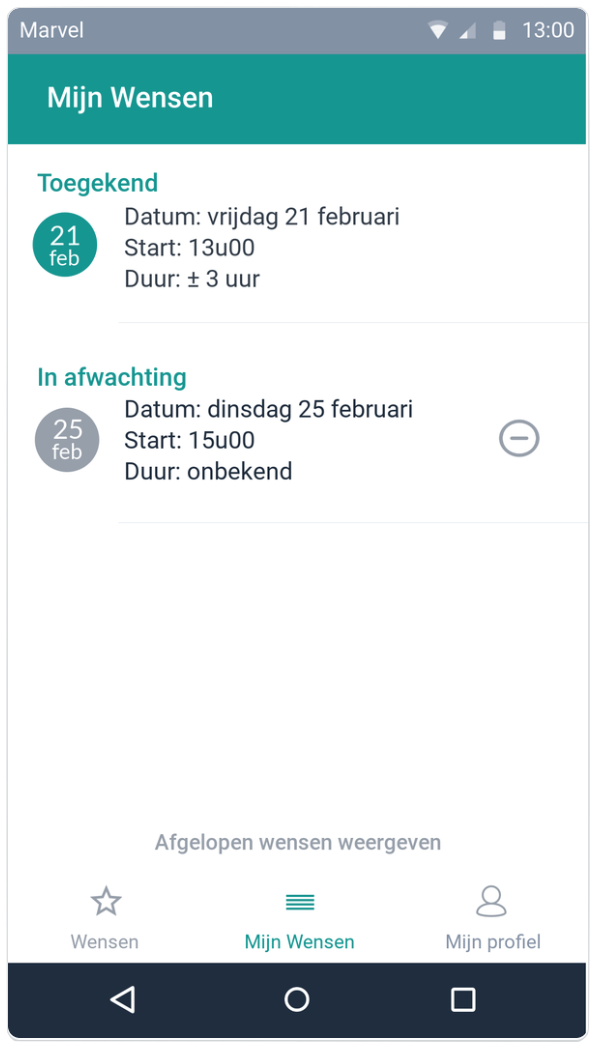
\includegraphics[width=0.685\textwidth]{images/care-athon/wensen.png}
  \end{subfigure}
  \begin{subfigure}[h]{0.3\textwidth}
    \centering
    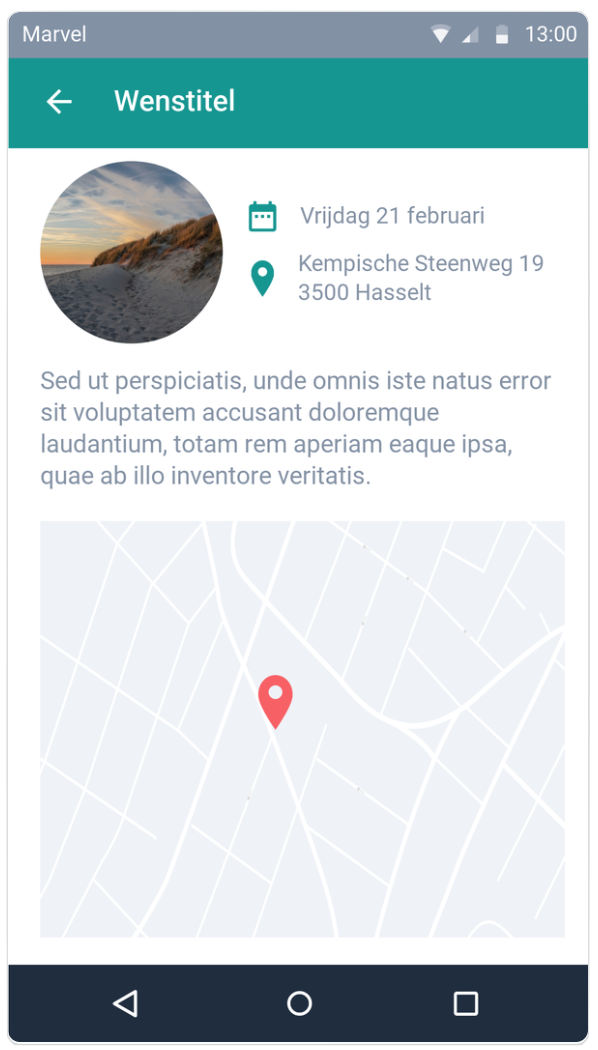
\includegraphics[width=0.685\textwidth]{images/care-athon/wens.png}
  \end{subfigure}
  \begin{subfigure}[h]{0.3\textwidth}
    \centering
    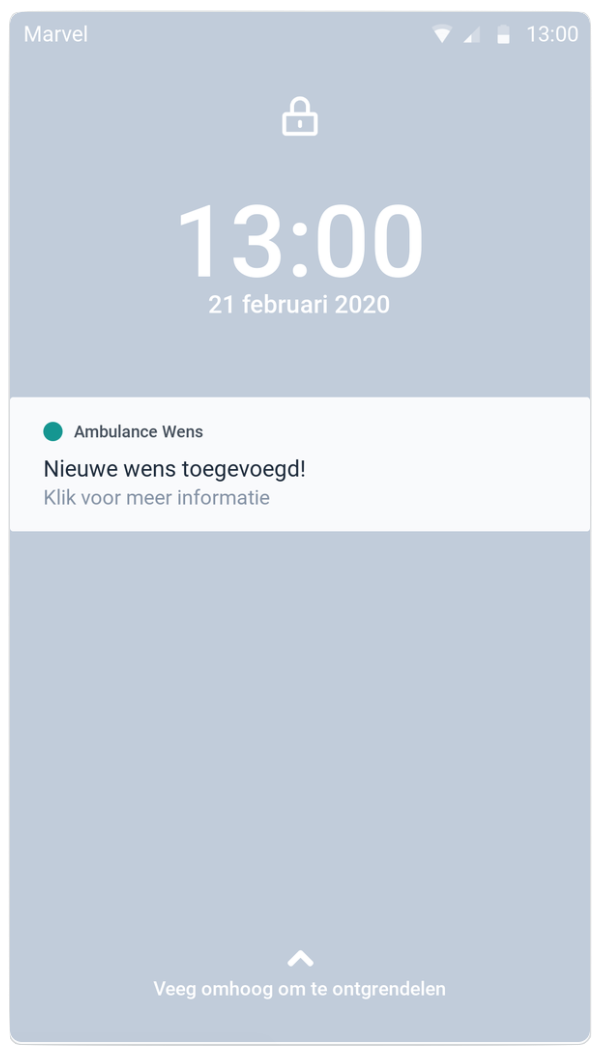
\includegraphics[width=0.685\textwidth]{images/care-athon/notificatie.png}
  \end{subfigure}
\end{figure}

\subsection{Studiereis: Berlijn (Technische Universit\"at Berlin)}
% htts://pxl-digital.pxl.be/page/studentenreis-2020-berlijn2

In de opleiding hoorde ook een deel over internationalisering uitgevoerd te worden. Hierdoor was er onder andere de mogelijkheid om op studiereis te gaan met medestudenten. Ik heb deze kans gegrepen en heb gekozen voor de studiereis naar Berlijn. Je kon kiezen tussen verschillende reizen. Er was er namelijk één naar Amsterdam en twee naar Berlijn. Die naar Amsterdam heb ik niet gekozen omdat ik de stad reeds vaker bezocht had en omdat het belangrijkste onderwerp van deze reis Cisco was, hetgeen mij niet echt aansprak. Bijgevolg bleven nog twee opties over waarbij ik het bezichtigen van de universiteit verkoos boven deelname aan de makathon.

De reis startte uiteraard met een lange busrit. Hier leerden we de groep wat beter kennen. Eenmaal aangekomen konden we inchecken in de kamer van het hotel en hadden we de rest van de avond nog vrij om Berlijn te gaan verkennen of om uit te rusten voor de drukke dagen die we tegemoet gingen komen.

Tijdens de eerste echte dag in Berlijn werden we opgesplitst in twee groepen om afwisselend de geplande activiteiten uit te voeren. Zo vertrok de ene groep naar de Stasi\hyp{}gevangenis Hohensch\"onhausen en de andere naar de Tempelhof luchthaven. In de namiddag wisselden de groepen van activiteit. In de gevangenis kregen we een rondleiding van een ex\hyp{}gevangene. Dit was zowel een voor\hyp{} als een nadeel. De spreker zijn Engels was niet erg goed waardoor hij initieel zeer moeilijk te verstaan was. Achteraf kon hij echter op een fascinerende manier zijn ervaringen en gevoelens delen met de groep, hetgeen zeker een meerwaarde vormde. Hij had een zeer fascinerende houding ten opzichte van de gevangenis en de bewakers van toen.

Daarna kregen we een rondleiding in de luchthaven, wat vroeger één van de grootste gebouwen van Europa was. Aangezien het een gigantisch gebouw omvatte, hebben we hier veel moeten wandelen, al was dit zeker en vast de moeite. De luchthaven was, toen wij hem bezochten, volledig leeg en verlaten, op een aantal ruimtes na. Dankzij de goede uitleg en aanvullende attributen kregen we toch een goed idee over hoe de luchthaven functioneerde gedurende zijn hoogtepunt en waarom dat hij zo goed bewaard is gebleven gedurende de oorlog. Ook werd aan ons verduidelijkt wat zijn huidige functie is en wat men in de toekomst nog ermee plande te doen.

De volgende dag was een toeristische rondleiding gepland in Berlijn. Zo reden we eerst met de bus door Berlijn en gaf een gids uitleg over monumenten en straten waar we langs of door reden. Na deze busrit gingen we te voet verder met de gids. Zo bezochten we bekende monumenten als de Berlijnse Muur, Checkpoint Charlie, Potsdamer Platz, de Berliner Dom, het Holocaust monument en nog veel meer. De gids gaf een goede uitleg over het verleden van deze monumenten maar ook de huidige betekenis en waarde ervan. Normaal gesproken ben ik geen grote voorstand van een rondleiding met een gids, maar door deze gids ben ik zeer aangenaam verrast omdat we veel hebben kunnen bezichtigen met een interessante uitleg en op korte tijd.

\begin{figure}[!h]
  \centering
  \begin{subfigure}[h]{0.48\textwidth}
    \centering
    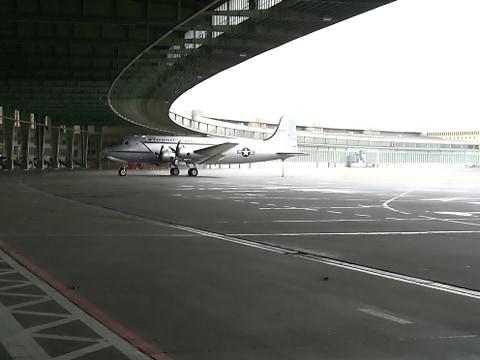
\includegraphics[width=0.85\linewidth]{images/berlijn/tempelhof.jpg}
    \caption{Tempelhof luchthaven}
  \end{subfigure}
  \begin{subfigure}[h]{0.48\textwidth}
    \centering
    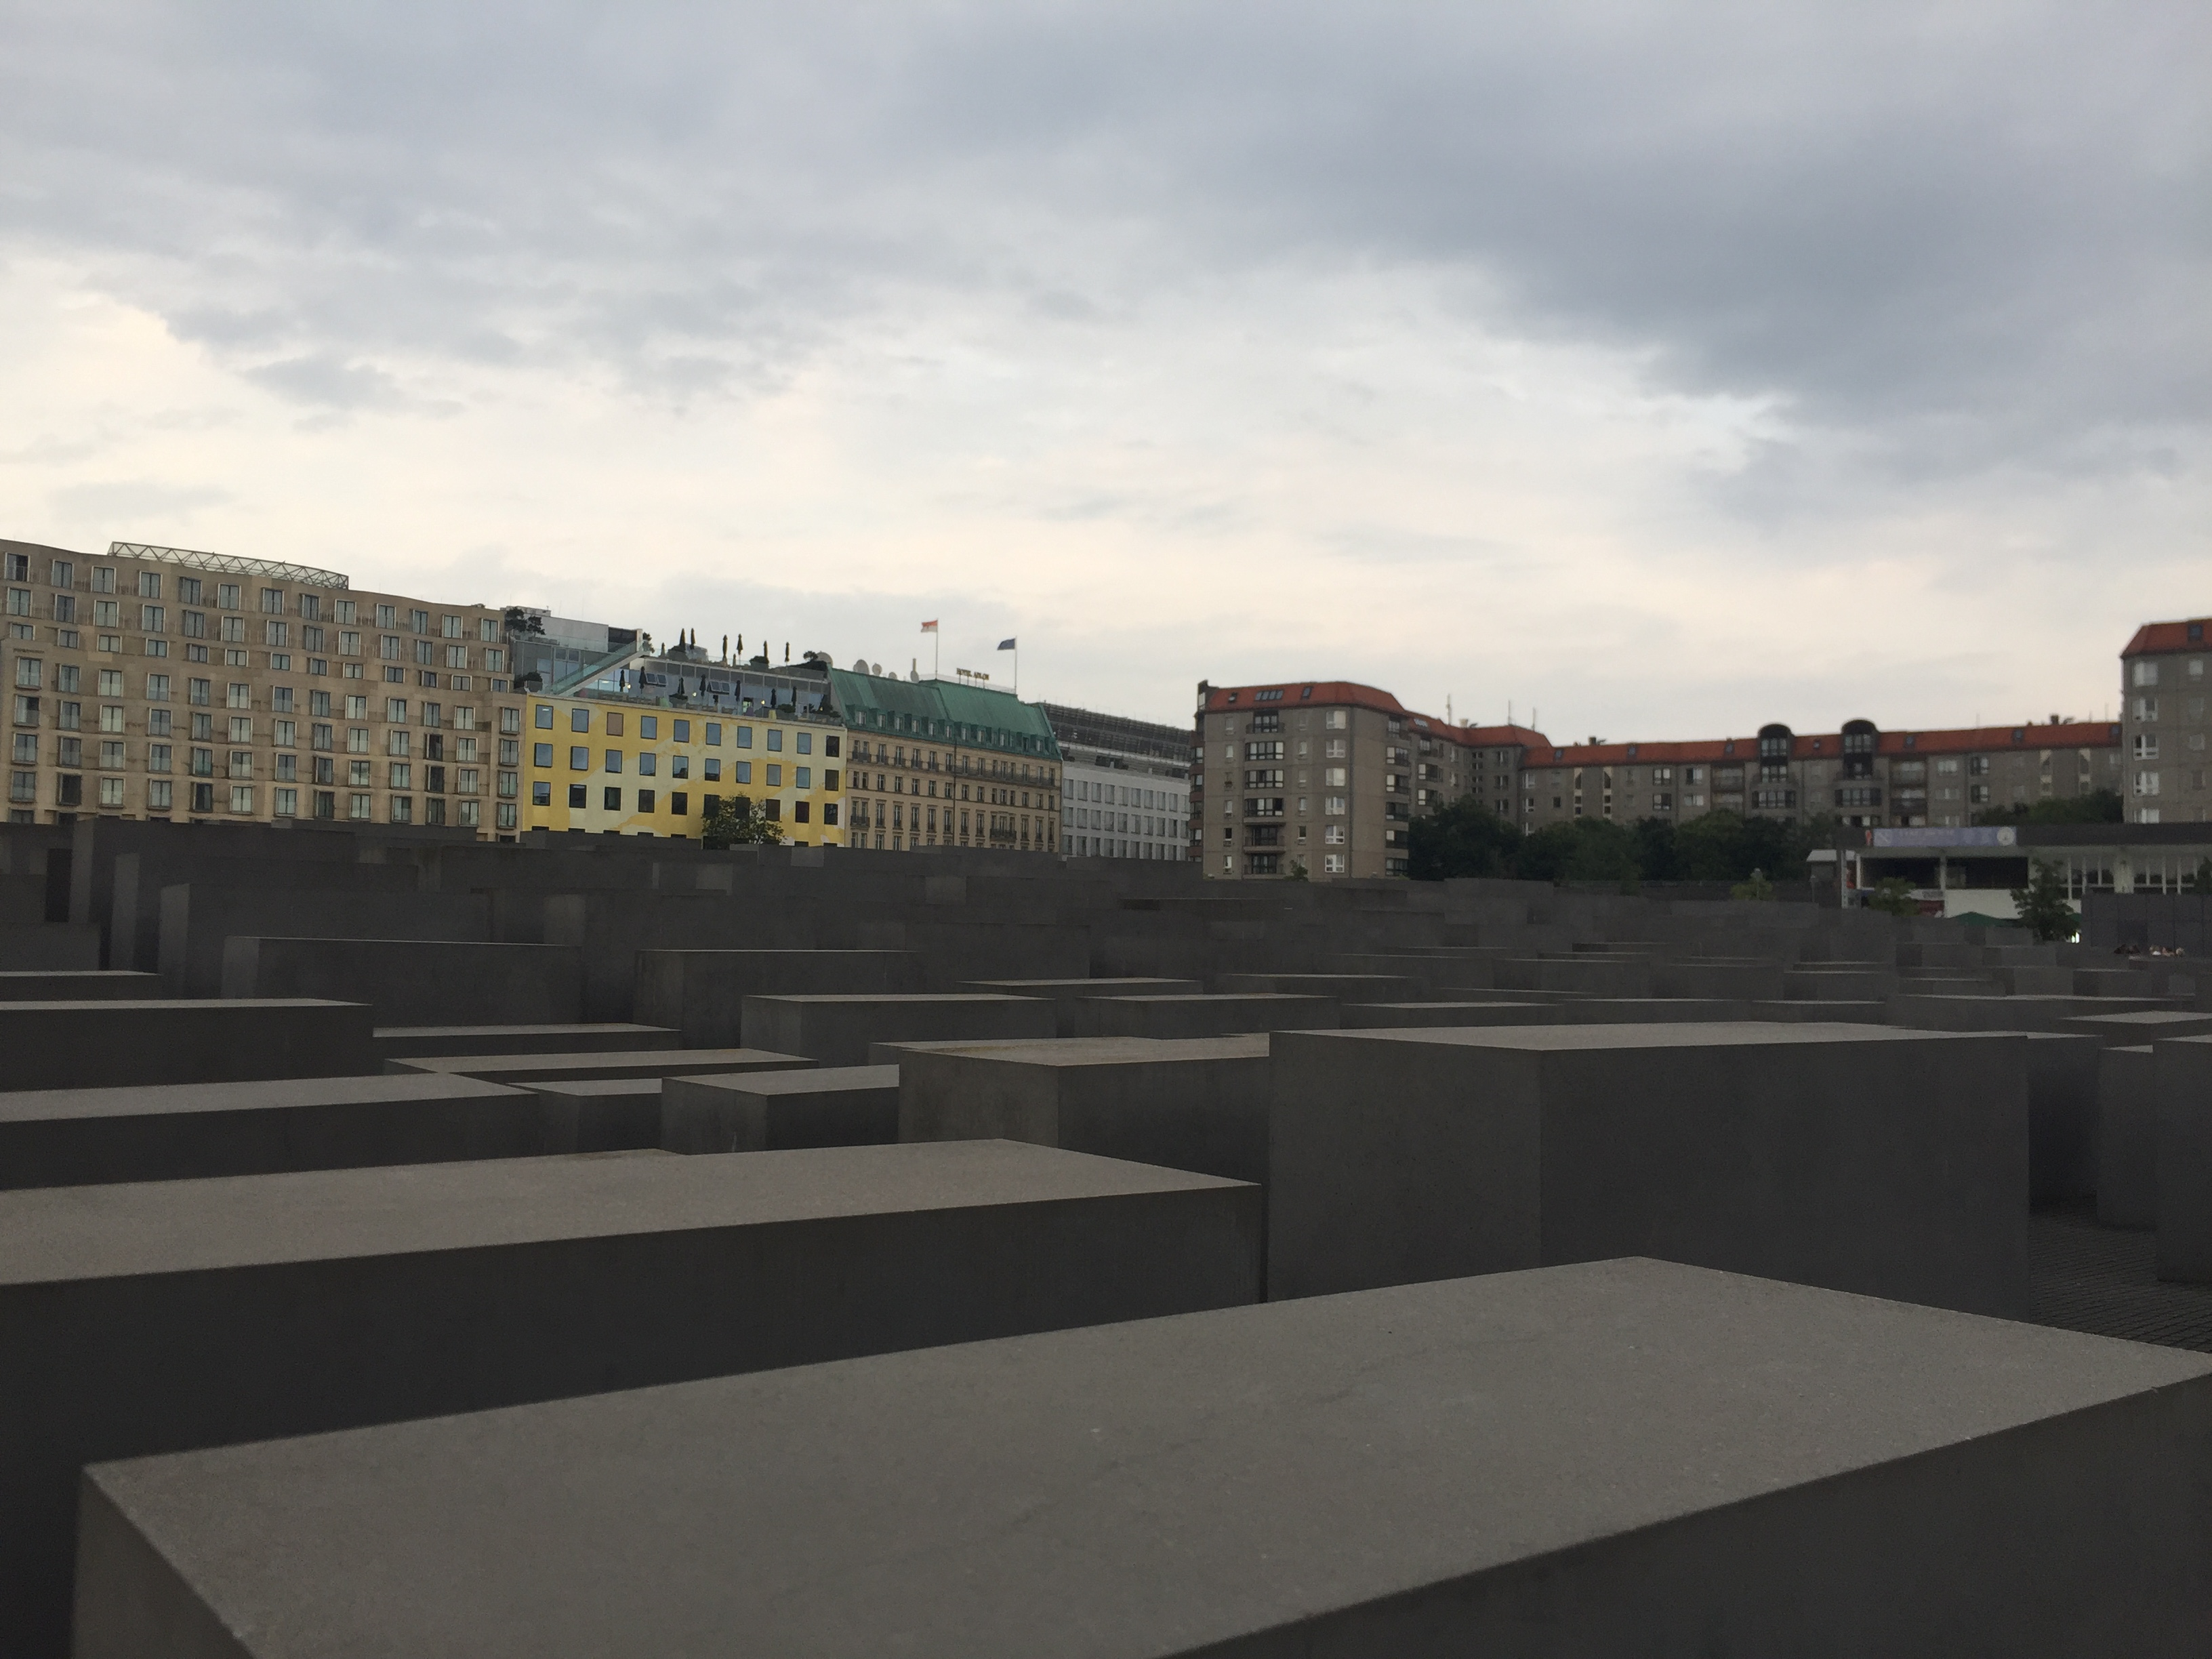
\includegraphics[width=0.85\linewidth]{images/berlijn/holocaust_monument.jpg}
    \caption{Holocaust monument}
  \end{subfigure}
\end{figure}

De laatste dag in Berlijn zouden we normaal naar de Technische Universit"at Berlin gaan en daar een seminarie volgen rond Future Security Lab, maar dit is niet door kunnen gaan omwille van een voor ons onbekende reden. Na de middag kregen we op diezelfde locatie normaalgezien ook een verrassingsseminarie, maar bijgevolg hebben we dit seminarie ook niet kunnen volgen. Omdat onze begeleiders deze late annulering niet hadden voorzien, mochten we de dag zelf inplannen. In groep zijn we Berlijn nog wat verder gaan verkennen en hebben we genoten van de stad. Ook hebben we kunnen uitrusten van de vermoeide afgelopen dagen. Na een korte nacht, zijn we uitgecheckt uit het hotel, hebben we ontbeten en zijn we de bus opgestapt richting Hasselt.

De studiereis was zeker geslaagd voor mij. Desondanks vond ik het jammer dat we niet naar de universiteit zijn kunnen gaan. Ik heb mijn medestudenten zeker beter leren kennen en nieuwe vrienden gemaakt, hetgeen ik vooraf niet had verwacht. De leuke groepssfeer maakte deze reis voor mij een unieke ervaring.

Op de onvoorziene omstandigheden na, zou ik de reis zeker opnieuw doen en aanraden aan de andere studenten. Het enige dat naar mijn mening minder aangenaam was, zijn de lange busritten, maar uiteraard horen ook zij erbij. Het was een vermoeiende reis door de relatief korte nachten en lange dagen, maar ook dit was het waard.

Ik heb deze opdracht opgenomen in mijn portfolio omdat deze studiereis een grote indruk heeft nagelaten op mij en het een groot deel uitmaakte van mijn derde en belangrijkste jaar op Hogeschool PXL. Ook omdat op gebied van mijn medestudenten leren kennen, dit toch een van de meest impactvolle elementen is en het plezier maken met elkaar.

\begin{figure}[!h]
  \centering
  \begin{subfigure}[h]{0.48\textwidth}
    
\includegraphics[width=\linewidth]{images/berlijn/berliner_dom.jpg}
    \caption{Berliner Dom}
  \end{subfigure}
  \begin{subfigure}[h]{0.48\textwidth}
    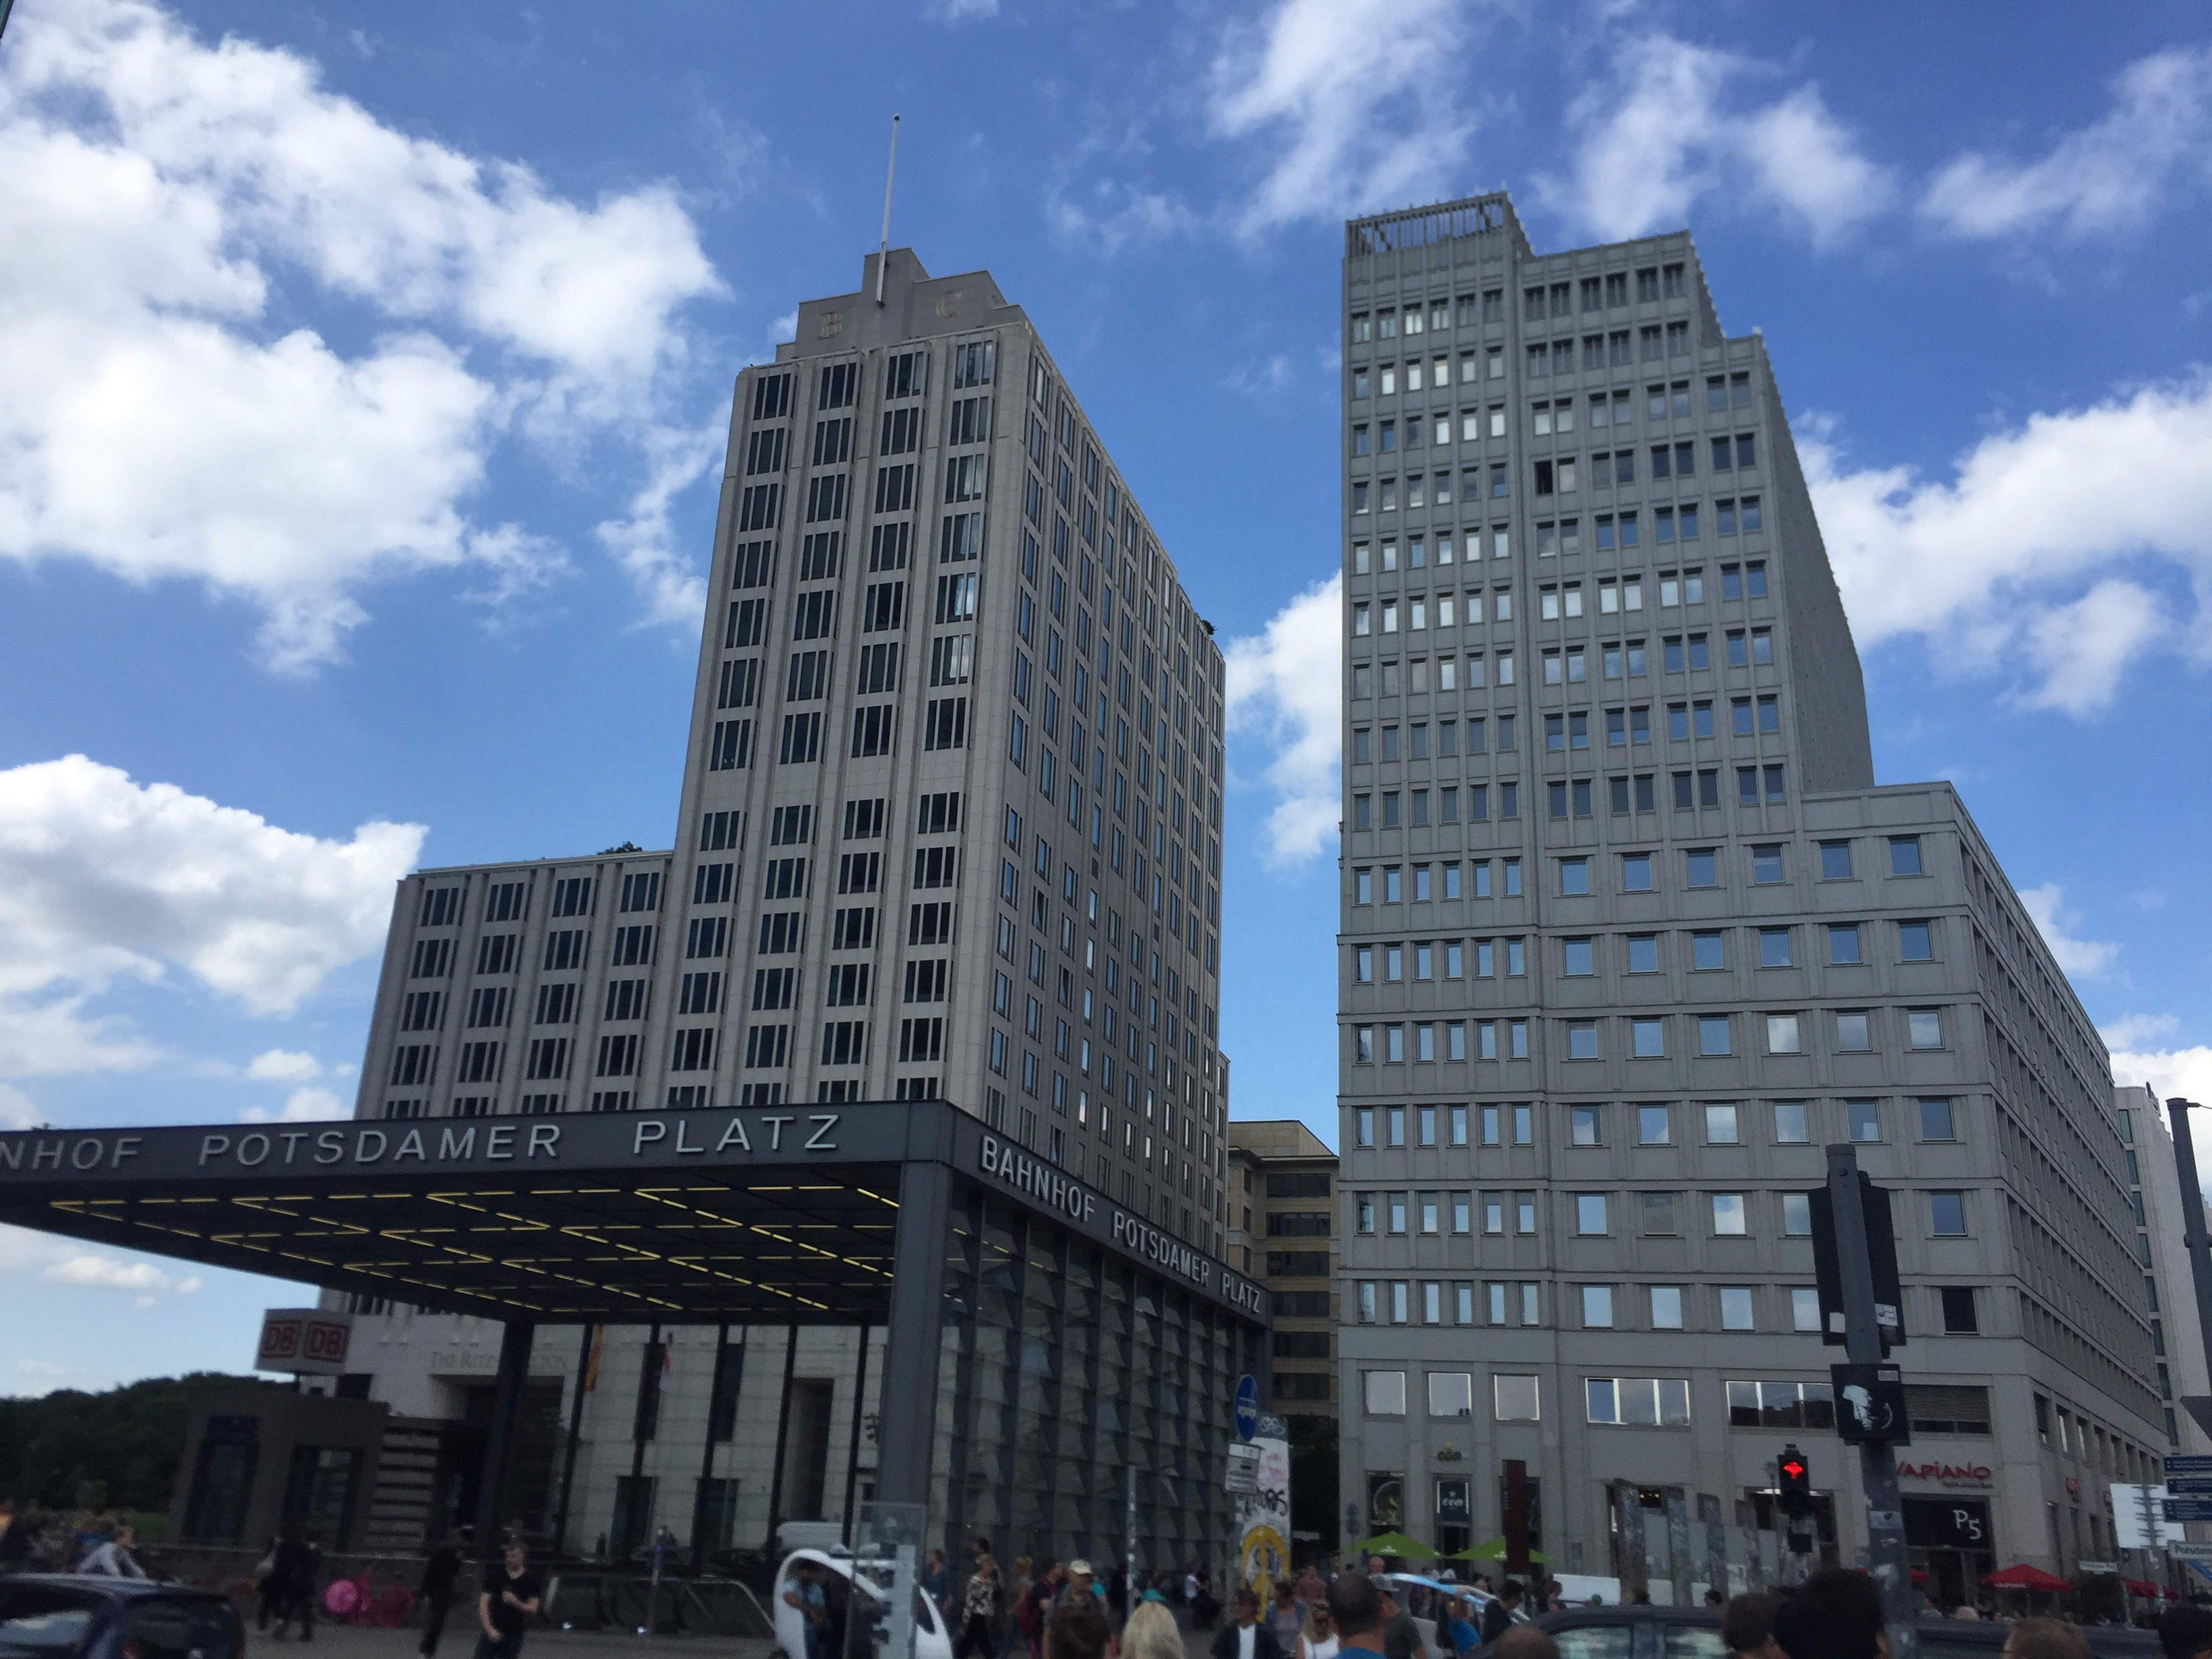
\includegraphics[width=\linewidth]{images/berlijn/potsdamer_platz.jpg}
    \caption{Portzdamer Platz}
  \end{subfigure}
  \begin{subfigure}[h]{0.48\textwidth}
    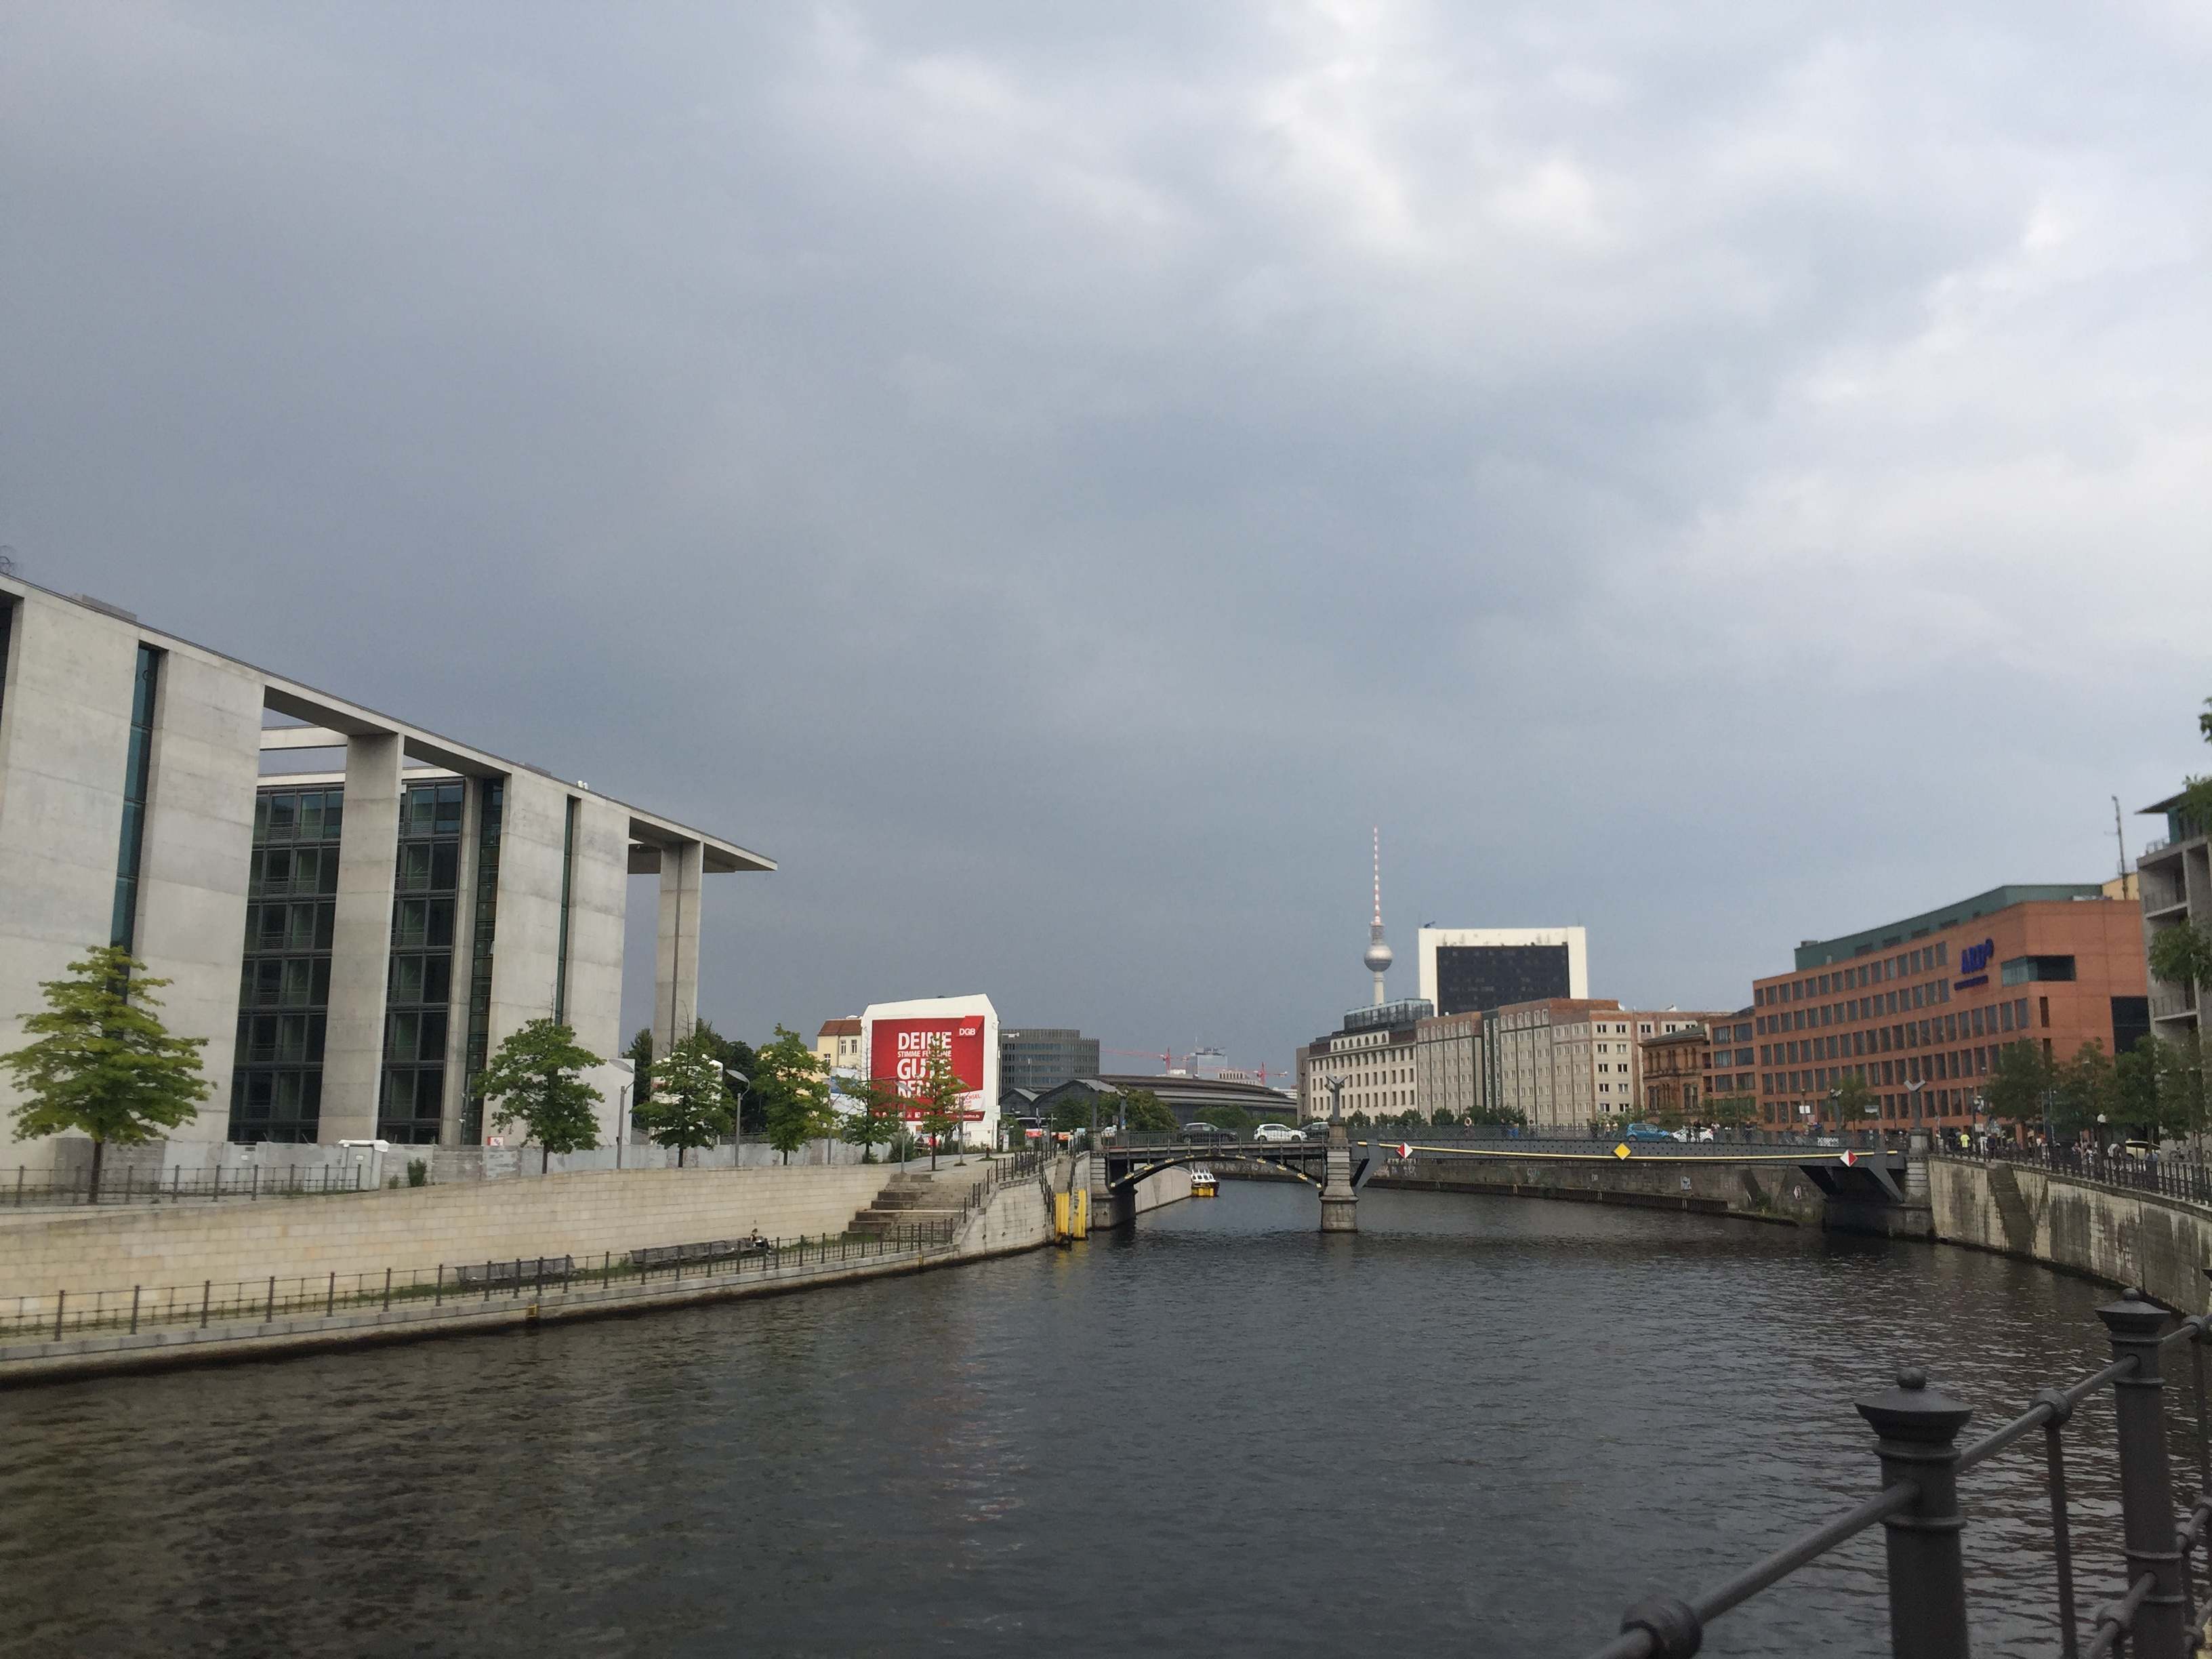
\includegraphics[width=\linewidth]{images/berlijn/uitzicht_reichstag.jpg}
    \caption{Uitzicht vanaf Reichstag}
  \end{subfigure}
  \begin{subfigure}[h]{0.48\textwidth}
    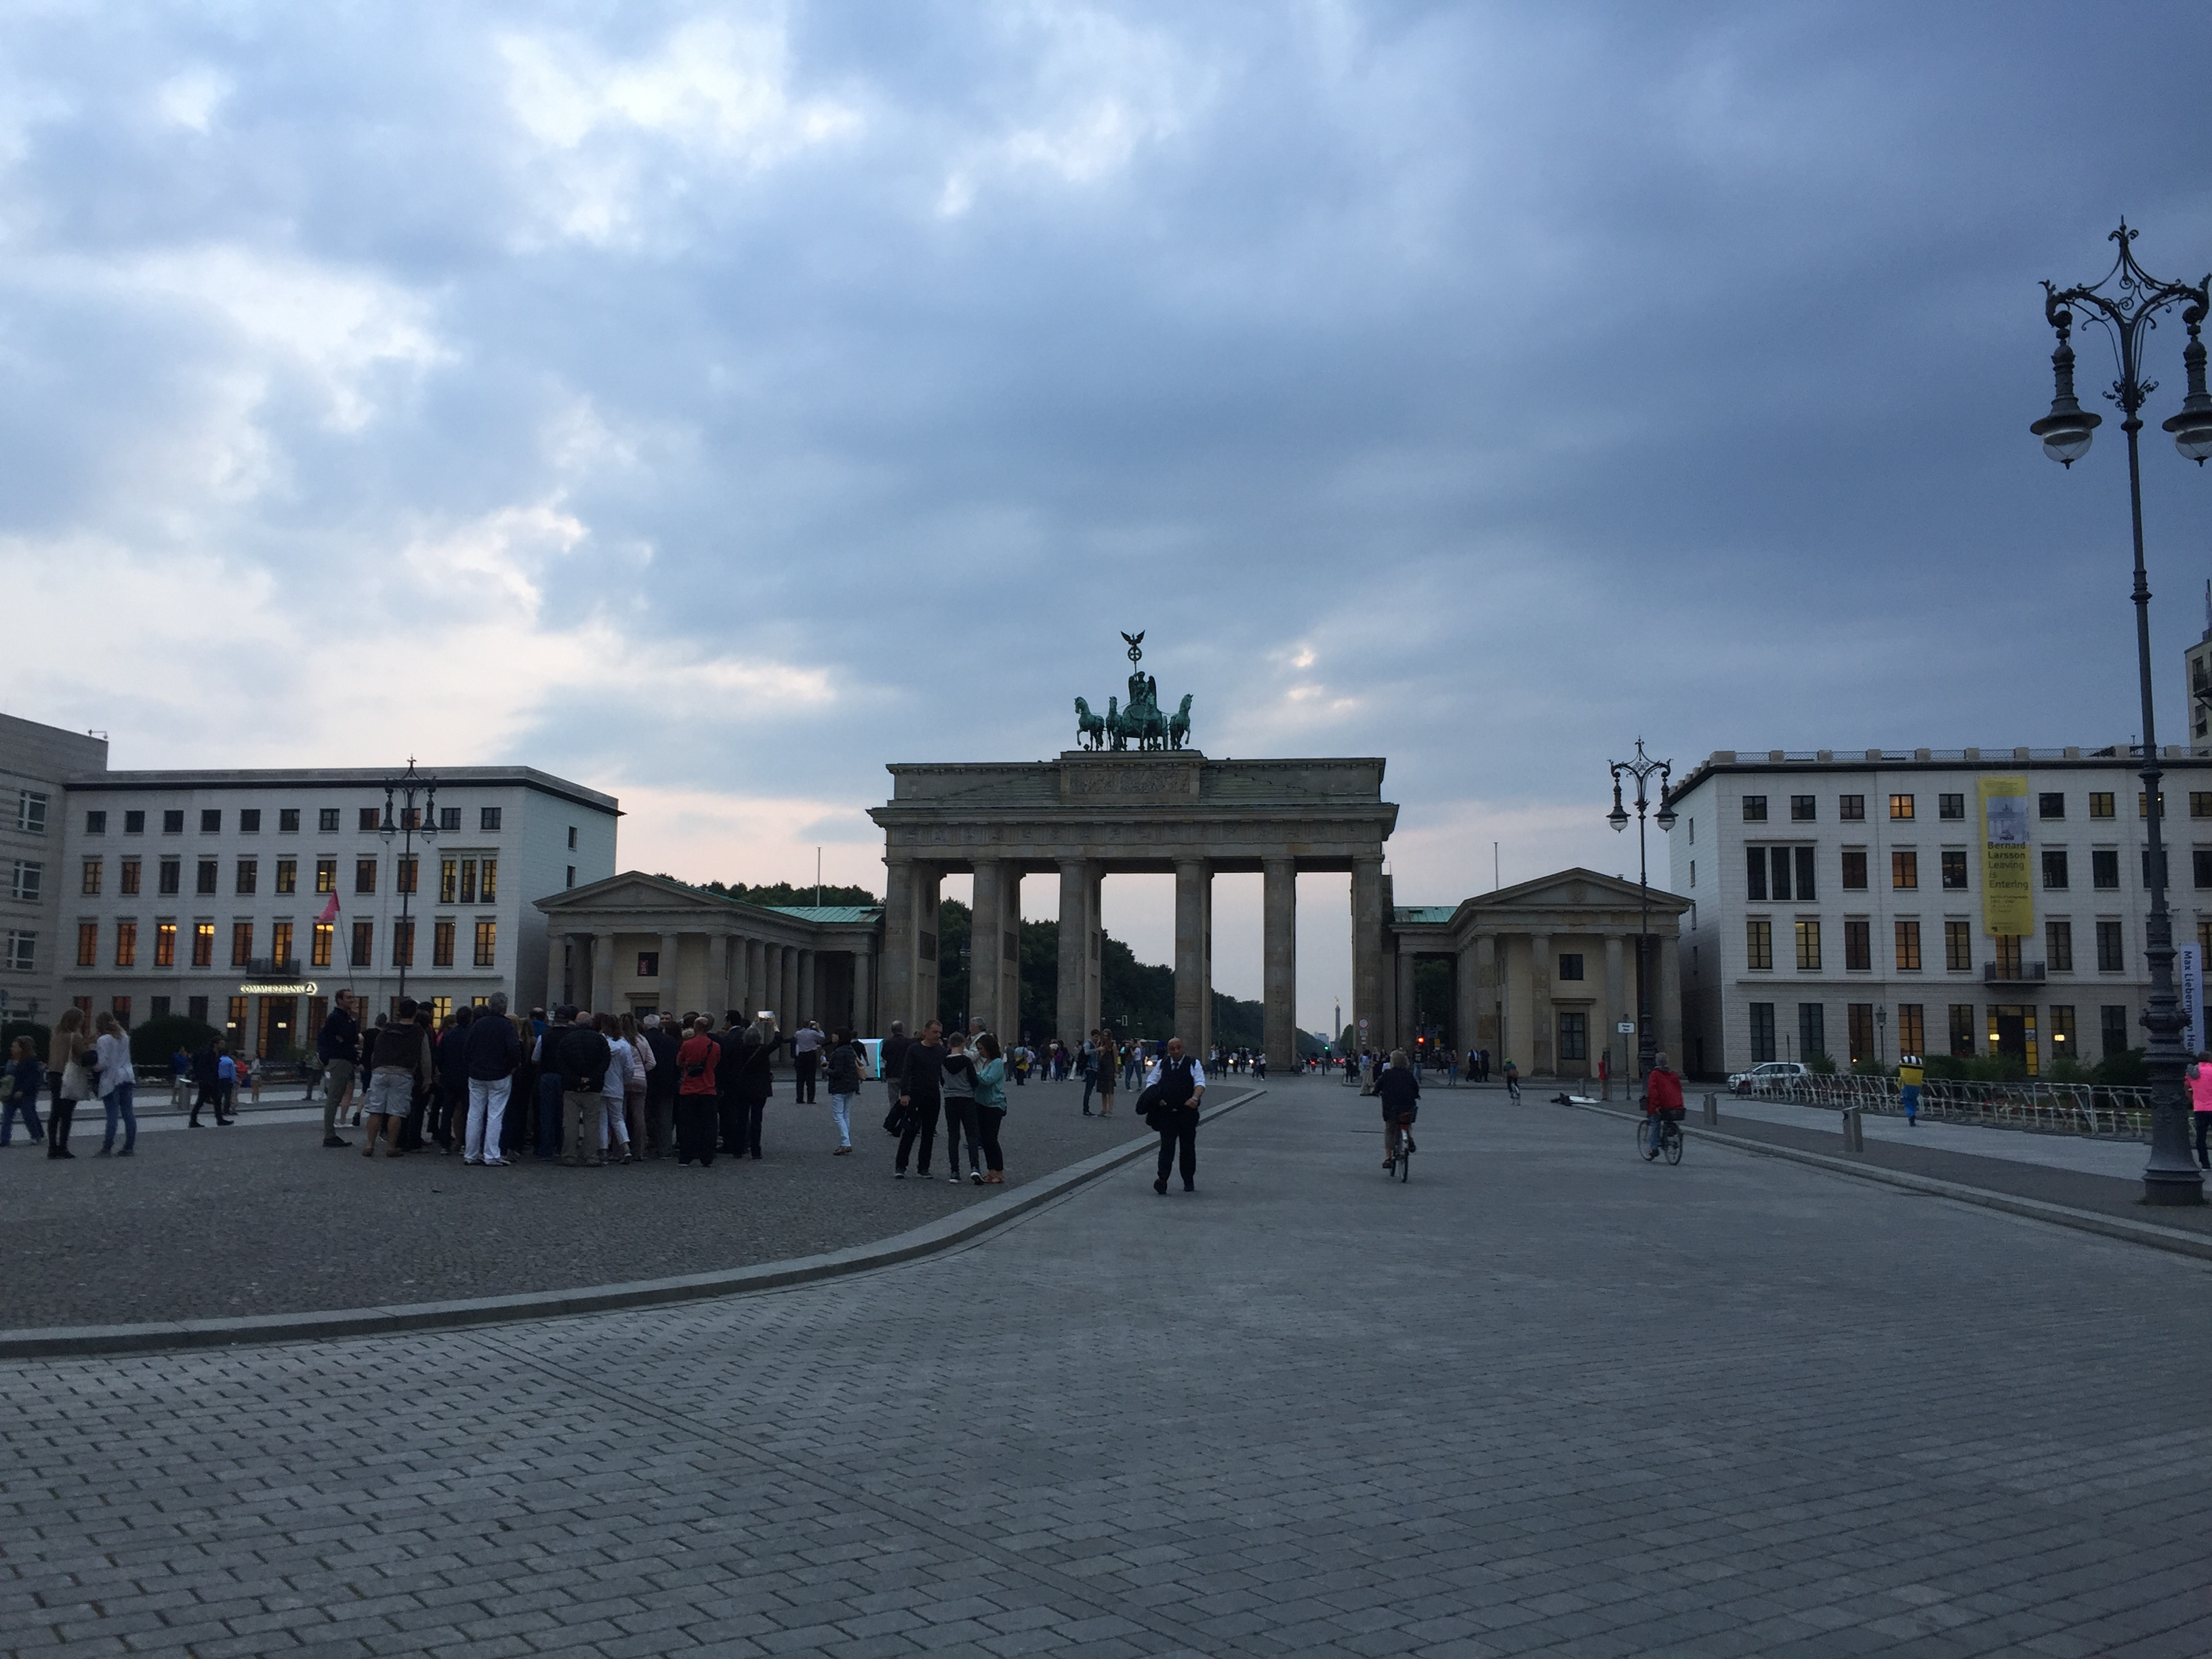
\includegraphics[width=\linewidth]{images/berlijn/brandenburger_tor.jpg}
    \caption{Brandenburger Tor}
  \end{subfigure}
\end{figure}

\subsection{AariXa - Docker for Dev and Ops}
% https://pxl-digital.pxl.be/page/seminarie-aarixa-27-02

Het eerste seminaire dat ik volgde voor iTalent ging over Docker, een tool om applicatie in containers te runnen. De spreker Sven Luts, softwareengineer bij AariXa, gaf uitleg over wat deze tool is, waarom het gebruikt wordt en hoe het achterliggend werkt. Hij maakte ook gebruik van demo's om de aangehaalde onderwerpen te verduidelijken.

In het begin stelde de spreker zich voor. Hij deelde zijn werkplek, zijn hobby's en zijn specialiteiten op gebied van informatica met ons. De introductie van Docker volgde zijn introductie. Docker is een tool gemaakt om het aanmaken, het deployen en het runnen van applicaties in containers te versimpelen.

Vervolgens gaf de spreker een uitleg over waarom je Docker moet gebruiken. Het vereenvoudigd niet alleen het maken en het deployen van software, maar het is ook veel sneller dan een virtuele machine. Het voorkomt de bekende uitspraak: "It works on my machine", dit bekomt Docker door in een afgeschermde en ge"isoleerde omgeving te werken. Deze omgeving bevatten alle benodigde dependencies en requirements. Docker bevat ook een ingebouwd version tracking door gebruik te maken van Docker tags. Een applicatie in een Docker container zal op eender wel systeem exact hetzelfde runnen ongeacht van de reeds ge"installeerde software op het host systeem.

Het volgende onderwerp was een Docker container, wat ze zijn en hoe je er aan kan komen. Een Docker container kan vergeleken worden met een virtuele machine, in de zin dat het ge"isoleerd is van het host systeem en het alle benodigdhede bevan die de applicatie nodig heeft om te runnen. Het verschil met een virtuele machine is dat een Docker container geen operating system moet gaan virtualiseren, wat een virtuele machine wel moet doen. Een Docker container gebruikt het operating system van het host systeem. Hierdoor is een Docker container beduidend kleiner is formaat dan een virtuele machine en heeft het praktisch geen opstarttijd.

Om een Docker container te bekomen is er eest een image nodig. Aan een Docker image kan je op twee manieren komen: je download het van het internet of je maakt er zelf een. Van een Docker registry kan een Docker image gepulld worden, dit is het equivalent van downloaden van het internet. De image kan ook zelf gebuild worden door het builden van een Dockerfile, een bestand waarin het buildproces van een image gedefinieerd wordt. Een Docker container verkrijg je als je deze Docker image runt. In een Docker container kunnen commits met veranderingen naar de image worden gedaan, waarna je deze Docker image weer naar een registry kan pushen.

De spreker toonde na deze uitleg hoe we Docker zelf konden installeren op ons systeem. Docker werkt achterliggend met Linux en vinden er geen problemen plaats bij een installatie op een Linux systeem. Als de installatie plaats vind op een Mac of een Windows systeem, gaat er in de achtergrond een virtuele machine met Linux opgestart worden die Docker beheert. Hierop volgde de uitleg van de basis commando's om Docker te beheren en monitoren.

\begin{figure}[!h]
  \centering
  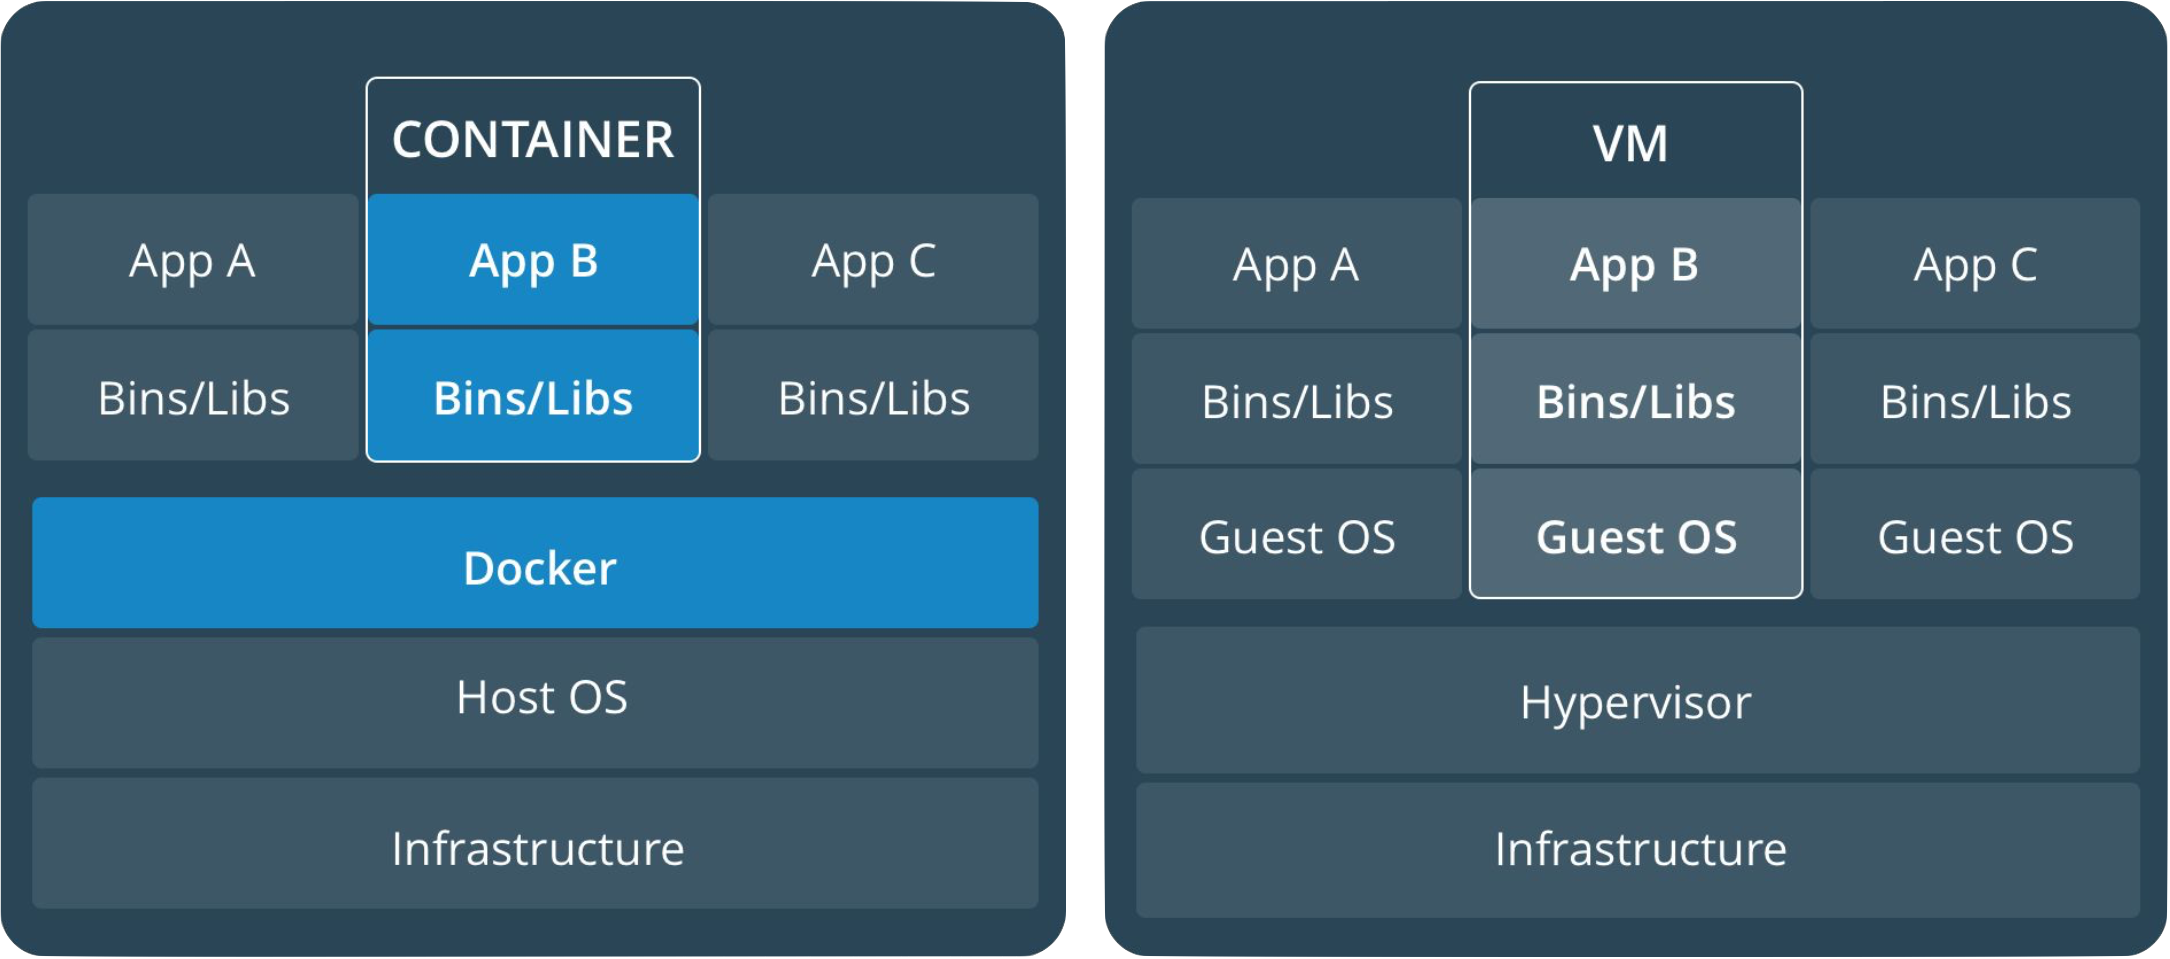
\includegraphics[width=0.72\linewidth]{images/docker/docker_vs_vm.png}
\end{figure}

Het seminarie sloot af met een korte demo over hoe we snel en gemakkelijk Docker commando's konden uittesten in een webapplicatie. Hiervoor moest er dus niets ge"installeerd worden. Deze demo functioneerde als de "Hello World!" van Docker. Na de demo gaf de spreker nog een kort vooruitzicht naar wat er in de toekomst met Docker kon gebeuren en gerealiseerd worden.

Het onderwerp van het gegeven seminarie vond ik boeiend, maar ik kon niet plaatsen hoe ik deze technologie zou kunnen gebruiken binnen mijn toekomstige projecten. Echter, toen ik gedurdende de vakken rond artifici"ele intelligentie en robotica in aanraking kwam met Docker, zag ik het nut van deze Docker in. Dit gaf mij niet alleen een grote voorsprong op mijn medestudenten die hier nog niet mee in aanraking gekomen waren, maar het deed mij ook beseffen dat het een zeer praktische technologie is waar ik in de toekomst ook nog gebruik van zou maken.

Ondertussen zijn mijn grootste projecten in Docker gemaakt. Namelijk mijn IT\hyp{}project en mijn stage hadden Docker als basis. Het seminarie en de technologie hebben mij ge"inspireerd om ge"isoleerde applicaties te gaan schrijven. Ook ga ik heel anders om met dependencies dan ik voordien deed, ik zorg dat ik altijd een stabiele versie van een bepaalde software gebruik en dat er geen conflicten zijn tussen de gebruikte software. Docker geeft in een bepaalde zin meer vrijheid om te experimenteren met het project. Doordat je altijd terug kan gaan naar een stabiele versie waarin de applicatie werkend is.

De spreker bracht deze presentatie zeer rustig en haalde goede punten aan. Door niet af te dwalen maar toch wat leuke weetjes in zijn presentatie te stoppen, verloor hij niemand zijn aandacht. Hij deelde zijn eigen ervaring met Docker. Zijn projecten konden zonder probleem op elke computer met Docker runnen, zonder dat hij hier enige extra moeiten in had gestoken.

Naar mijn mening is Docker zo handig dat ik het in een laat eerste of vroeg tweede jaars vak aan zou halen. Dit kan makkelijk in vakken zoals Desktop OS of Server OS Essentials, waar we al kennis maakten met Linux. De tijd die ik al gewonnen heb met Docker en de vrijheid die je er van krijgt, zorgen ervoor dat Docker momenteel een van mijn favoriete en meest gebruikte technologie is.

Spreker: Sven Luts, software engineer bij AariXa, \url{https://be.linkedin.com/in/svenluts/nl}


\begin{figure}[!h]
  \centering
  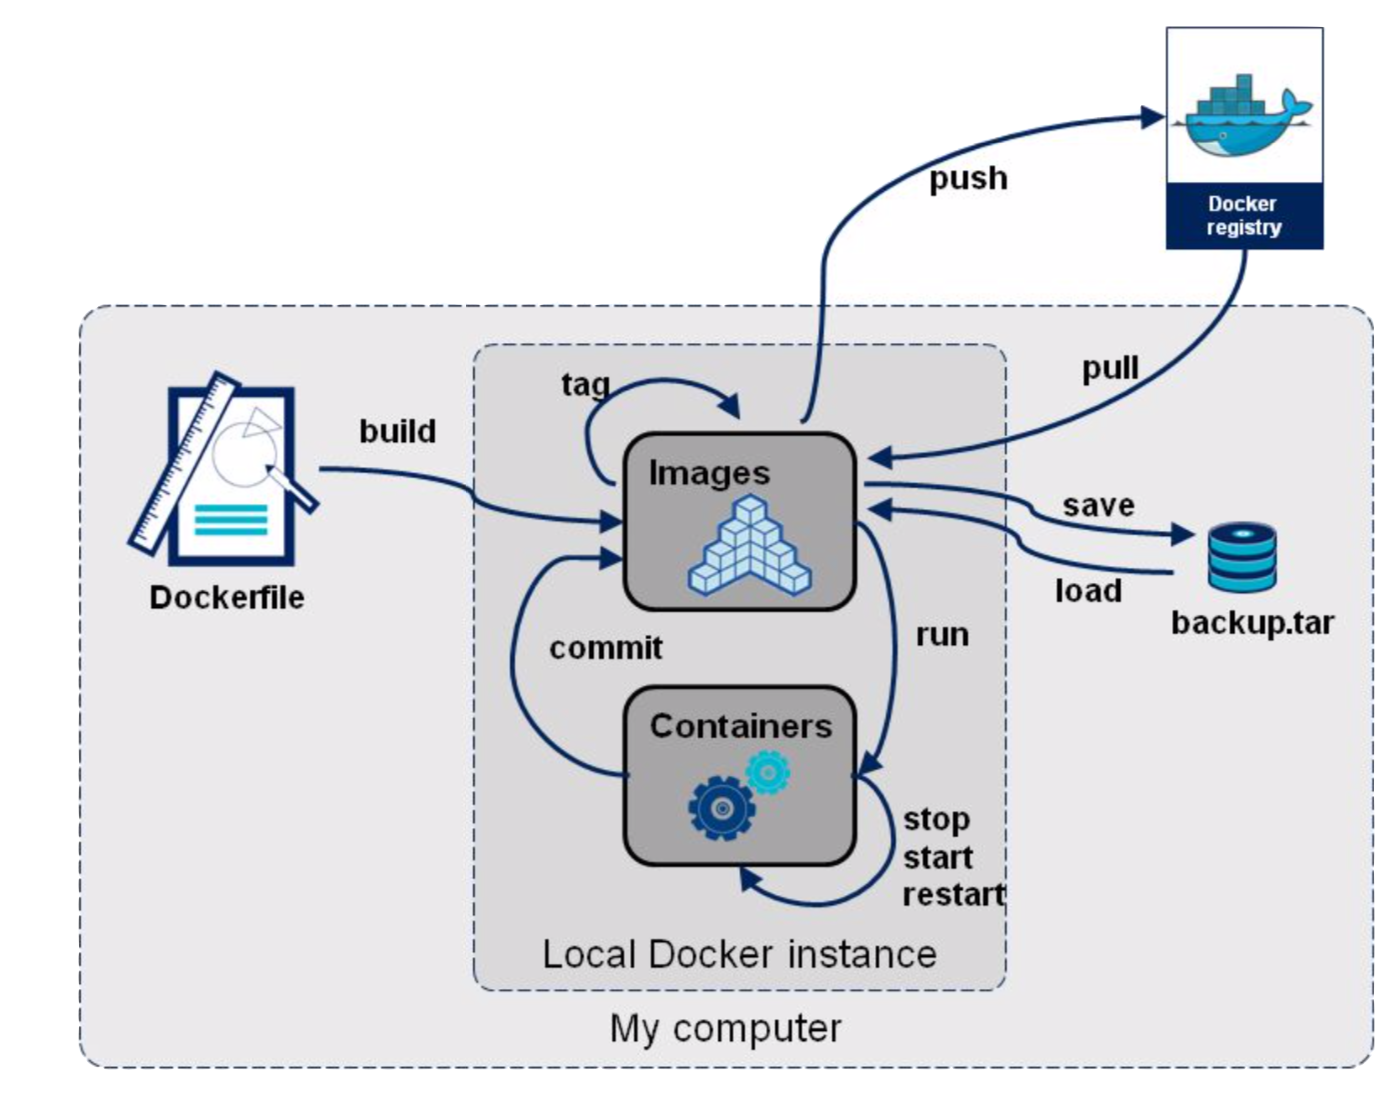
\includegraphics[width=0.74\linewidth]{images/docker/flow.png}
\end{figure}

\subsection{\LaTeX{} - Softwaresysteem voor het zetten van documenten}
\LaTeX{} is een softwaresysteem vergelijkbaar met een tekstverwerker zoals Microsoft Word. In de wetenschappelijke wereld is dit een zeer populaire software omdat het uitblinkt in het maken van technische documenten. \LaTeX{} is een markup\hyp{}taal.

Ik kwam als eerste in contact met \LaTeX{} door de standaard tekstverwerker van Mac, genaamd Pages. In deze tekstverwerker kan je wiskundige formules toevoegen in een \LaTeX{}\hyp{}notatie. Ik probeerde de code die ik online vond te ontleden en kon zo mijn eigen wiskundige formules schrijven in deze taal.

Later kwam ik er achter dat \LaTeX{} niet enkel een gebruikt kan worden voor wiskundige formules, maar dat het ook als volwaardige tekstverwerker kan functioneren. Omdat zeer veel papers geschreven worden met \LaTeX{}, besloot ik om mijn eindwerk ermee te schrijven. Dit zorgde dat ik meer onderzoek moest gaan doen naar hoe ik dit kon realiseren.

\LaTeX{} is het meest gebruikte macropakket van \TeX{}. \TeX{} is ontwikkeld in de jaren 70 door Donald Knuth om op een relatief eenvoudige manier het beschrijven van een ingewikkelde lay\hyp{}out mogelijk te maken. \TeX{} en dus ook \LaTeX{} zijn WYMIWYG, "What you mean is what you get", in tegenstelling tot andere WYSIWYG, "What you see is what you get", tekstverwerkers. Net zoals computerprogramma's moet een \TeX{}\hyp{}document gecompileerd worden om het resultaat te krijgen. De conventie is het compileren naar een pdf\hyp{}bestand.

De macro's in het \LaTeX{}\hyp{}pakket zijn voorgedefinieerde combinaties van commando's om het opmaakproces te versnellen. De schrijver kan deze macro's niet alleen gebruiken, maar zo ook aanpassen zijn zijn precieze nood. De mogelijkheid tot het schrijven van eigen macro's is natuurlijk ook een optie.

Het gehele idee achter het opmaken van een bestand in \LaTeX{} is dat je op voorhand bepaalde regels definieert en je gedurende het hele schrijfproces, je geen rekening meer moet houden met de opmaak. Zo krijg je een consistente lay\hyp{}out doorheen je bestand zonder al te veel moeite. Het versimpelt ook het wijzigen van de lay\hyp{}out omdat het op één globale plaats staat gedefinieerd.

Als oefening begon ik met het namaken van de gekregen templates voor documenten tijdens de stage in \LaTeX{}\hyp{}formaat. Deze documenten waren: het stageportfolio, de projectomschrijving en uiteindelijk het eindwerk zelf. Opdat ik meer met de taal werkte en meer onderzoek ernaar deed, kwam ik regelmatig op bevindingen die ervoor zorgde dat mijn hele structuur veranderde. Maar deze veranderingen zorgden er iedere keer voor dat het opmaakproces makkelijker en makkelijker werd.

\begin{figure}[!h]
  \centering
  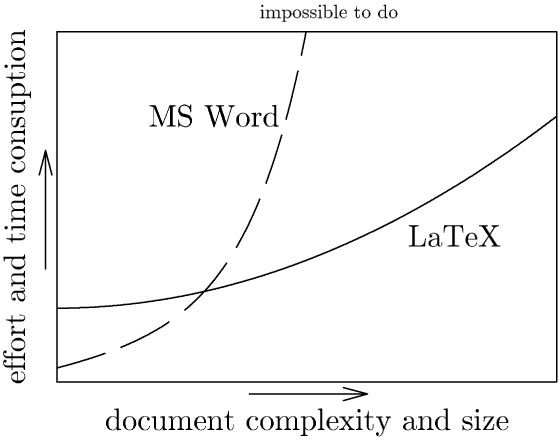
\includegraphics[width=0.48\linewidth]{images/latex/ms_word_vs_latex.png}
\end{figure}

\LaTeX{} heeft naar mijn mening een redelijk steile leercurve, maar eenmaal hier over kan je  er de vruchten van plukken. Voor de opmaak van mijn stageportfolio en mijn projectomschrijving heb ik wat meer tijd gestoken in vergelijking dat ik het met een tekstverwerker deed die ik reeds kende. Maar voor het eindwerk van de stage en het portfolio van iTalent heeft dit zeer veel tijd uitgespaard omdat ik praktisch geen rekening meer moest houden met het maken en volgen van de lay\hyp{}outregels.

Het idee achter het schrijven van mijn eindwerk in \LaTeX{} is dat ik na mijn bacheloropleiding wil doorschakelen naar een masteropleiding. Hier ga ik een master thesis voor moeten schrijven en om mij zo veel mogelijk te kunnen concentreren op het effectief schrijven en niet zo zeer op het opmaken van het document, zou ik deze in \LaTeX{} schrijven. Het lijkt mij ook een goed idee, want er worden veel master thesissen geschreven in \LaTeX{}. Dus het mijn eindwerk van mijn bacheloropleiding is de ideale voorbereiding voor mijn master thesis.

Nog een groot voordeel dat ik voordien niet wist is het gebruik van Bib\TeX{}. Dit is een soort van extensie op \LaTeX{} voor het aanleggen van literatuurlijsten. Google Scholar, een internetzoekmachine voor wetenschappelijke teksten en artikels, heeft een functie waarmee het gezochte bronnen kan citeren in een Bib\TeX{}\hyp{}formaat. Zo hoef je zelf niet alle informatie uit dit artikel of deze tekst te halen.

Het leren van \LaTeX{} is voor mij zeer nuttig geweest. Ik heb hierdoor een andere kijk gekregen op het maken en opstellen van tekstdocumenten. In het algemeen verlies ik veel minder tijd met het opmaken en het verfijnen van de opmaak. Ook het toepassen van mijn opmaak gebeurt nu automatisch. Hierdoor heb ik meer tijd om te spenderen aan het effectief schrijven van de tekst. Niet alleen het document maar ook de achterliggende structuur is voor mij nu overzichtelijker en makkelijk te lezen.

Doordat ik nieuwsgierig ben van karakter, vind ik het spannend om nieuwe technologi"en te onderzoeken en te leren. Niet alleen om mijn kennis te verruimen en te groeien als informaticus, maar ook omdat ik er vaak positieve zaken uit haal die ik initieel niet had verwacht. Mijn doel is om zo performant mogelijk te werken en dus zo weinig mogelijk tijd te verliezen met zaken die in mijn ogen niet nodig zijn. Met deze attitude zoek ik naar nieuwe technologi"en die mij verder kunnen helpen dit te bereiken. Ook mijn eigen uitdagen op zulke projecten geeft mij meer motivatie om er zo veel mogelijk uit te halen en is het voor mij geen moeite om er veel tijd in te steken.

Broncode iTalent portfolio: \url{https://github.com/VicSegers/iTalent-portfolio}
